\documentclass{article}

\usepackage[utf8]{inputenc}
\usepackage{geometry}
\usepackage{graphicx}
\usepackage{titling}
\usepackage{fancyhdr}
\usepackage{cmbright}

\geometry{
	a4paper,
	total={170mm, 257mm},
	left=20mm,
	top=20mm
}



\title{Chapter 2: Vehicle 2 - Fear and Agression}
\author{Fharook Shaik}
\date{12 November 2024}

\fancypagestyle{fancy}{
	\fancyhf{}
	\fancyfoot[R]{
\includegraphics[width=3cm]{images/BTULogo_englisch_grau_2x.png}}
	\fancyfoot[L]{\thedate}
	\fancyhead[L]{13869 - Braitenberg Vehicle Praktium}
	\fancyhead[R]{\theauthor}
}

\pagestyle{fancy}

\makeatletter
\renewcommand{\maketitle}{
	\thispagestyle{fancy}
	\null
	\vskip 1em
	\begin{center}
		{\LARGE \@title \par}
	\end{center}
	\vskip 3em
}
\makeatother


\begin{document}

	\maketitle

	\noindent\begin{tabular}{@{}ll}
		Student & \theauthor\\
		Professor &  Dr. Cunningham, Douglas\\
		Matrikel-Nr.: & 5014962
		 
	\end{tabular}

	\section*{Summary}
	Building on Chapter 1's idea that the vehicle is \textit{Atleast Alive}, Chapter 2 of \textbf{Vehicles: Experiments in Synthetic Psychology} by \textit{Valentino Braitenberg} introduces Vehicle 2, an upgraded version of his basic vehicles that seems to display emotions like fear and aggression. Vehicle 2 is similar to the first one, but now it is equiped with two sensors and two motors, one on each side. This new setup allows Vehicle 2 to behave in more complex ways, which Braitenberg compares to emotions.

	Braitenberg explains that Vehicle 2 is like a "descendant" of Vehicle 1, almost as it two of the simpler models were fused together. Braitenberg tries out three wiring options for how the sensors control the motors.

	\begin{figure}[h]
		\centering
		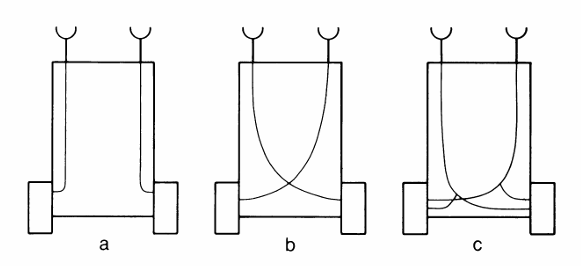
\includegraphics[scale=0.6]{images/Vehicle 2 Setups.png}
		\caption{Vehicle 2 (a) Same Side wiring (b) Opposite-Side wiring (c) Both side wiring }
		\label{fig:vehicle-2_setup}
	\end{figure}

	\subsection*{Same-Side wiring (Vehicle 2a)}
	In this setup, each sensor controls the motor on the same side. If the vehicle faces a source (like a light source) directly upahead, it moves toward it with its speed gradually increasing. But if the source is off to one side, the sensor of that side kicks in the motor of the same side, turning the vehicle away from the source such as \textit{fleeing} from it. This gives Vehicle (2a) a \textbf{fearful} personality that avoids strong sources and stays in areas of source with low to none impact, looking \textbf{Cowardly} as it tries to escape from it.

	\subsection*{Opposite-Side wiring (Vehicle 2b)}
	In this setup, each sensor controls the motor on the opposite side. Similar to Vehicle (2a) behaviour, Vehicle (2b) also moves towards the source if it is located directly upahead. Either the vehicle or source is deflected from other, the vehicle always reorient towards the source and end up hitting it. This creates an \textbf{Aggressive} behaviour, as Vehicle (2b) repeatedly moves towards the source, colliding with it as if it is trying to destroy it. 

	\begin{figure}[h]
		\centering
		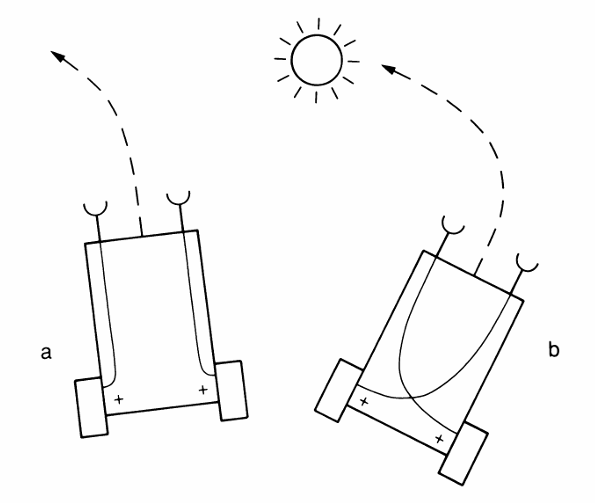
\includegraphics[scale=0.6]{images/Vehicle 2 Behaviour.png}
		\caption{Vehicle (2a),(2b) Behaviour }
		\label{fig:vehicle-2_behaviour}
	\end{figure}

	\subsection*{Both sensors to Both motors (Vehicle 2c)}
	This option is dismissed because it behaves like an upgraded version of Vehicle 1 with double the sensors and motors. 

	\newpage

	Braitenberg's key idea is that, with these simple setups, the vehicles seem to show emotions: Vehicle 2a "fearful" act in avoiding the source, while Vehicle 2b "aggressive" act repeatedly charges at the source. These behaviours make Vehicle 2 seem more \textbf{emotionally intelligent} because it's reacting in ways that look purposeful or even lifelike. 

\end{document}